% Capítulo 2 - vFinal 1.0 - 05/07/2018
\chapter{Conceitos Relacionados}
\label{cap:cap2}

Este capítulo aborda os conceitos e técnicas que proporcionam a compreensão dos capítulos a seguir. A Seção \ref{cap2:energyDriven} introduz o conceito da computação dirigida aos fatores energéticos, tema originador do trabalho. Na Seção \ref{cap2:iot}, apresento a visão geral sobre Redes IoT e dispositivos que compõe o alvo das iniciativas propostas. Por sua vez, na Seção \ref{cap2:throttling} encontram-se os conceitos ligados ao padrão throttling, seu conceito e sua aplicação. A intenção de uso de um modelo taxonômico esta fundamentada na Seção \ref{cap2:taxonomia}.

\section{Energy-Driven Computing}
\label{cap2:energyDriven}

Um sistema dirigido à energia (\textit{Energy-Driven}), é todo aquele que os fatores energéticos intrínsecos a ele são tratados como primários, desde concepção, gerenciamento e sua operação \cite{merrett_energy-driven_2017}. Computação dirigida a estes fatores, ditos energéticos, deve considerar fundamentalmente a disponibilidade energética pois precisam carregar a capacidade de adaptação as dinâmicas de captação de energia. Este paradigma tem como objetivo evidenciar as características energéticas, em potencial a respeito de dispositivos que por quaisquer motivos, não podem estar conectados diretamente em uma infraestrutura capaz de fornecer energia virtualmente ilimitada. 

Para tal, caso necessário, dispositivos podem operar coletando recursos disponíveis no ambiente. Coleta de energia refere-se a capacidade de um dispositivo em capturar e converter recursos energéticos do meio e converte-los de modo a prolongar sua vida útil mitigando um cenário de escassez energética \cite{sudevalayam_energy_2011}. 

Ainda, no trabalho de \cite{sliper_energy-driven_2020} é importante destacar como os mecanismos de coleta energética e sua dinâmica são dispostos. É proposto uma organização em três categorias distintas: Neutra-Energética \ac{EN}, Neutra-Força ou Neutra em Consumo \ac{PNO} e por fim, Operações Intermitentes.

\subsection{Operação Energy-Neutral}
Uma operação neutra-energética \cite{kansal_power_2007}, cobre as dinâmicas dos sistemas com coleta de energia do ambiente por meio de um \textit{buffer}, uma bateria recarregável ou super capacitor capaz de armazenar parte da energia coletada. Este recurso, se encontra disposto entre a entrada energética e sua demanda, atuando secundariamente quando a energia disponibilizada não seria suficiente para manter seus critérios de qualidade de serviço \textit{QoS}.

Apesar de inicialmente ser previsto um cenário de uso onde apenas a fonte energética e o dispositivo estivessem presentes, é comum o fato dos mecanismos que buscam esse tipo de operação recorrer a presença deste componente intermediário capaz de armazenar energia e disponibiliza-la para uso. Sendo assim, na Figura \ref{fig:cap2harveststoreuse} temos a visão geral em blocos de um subsistema responsável pelos recursos energéticos.

\begin{figure}[H]
	\centering
	\caption{Diagrama de blocos subsistema energético para operação neutro-energética.}
	\label{fig:cap2harveststoreuse}
	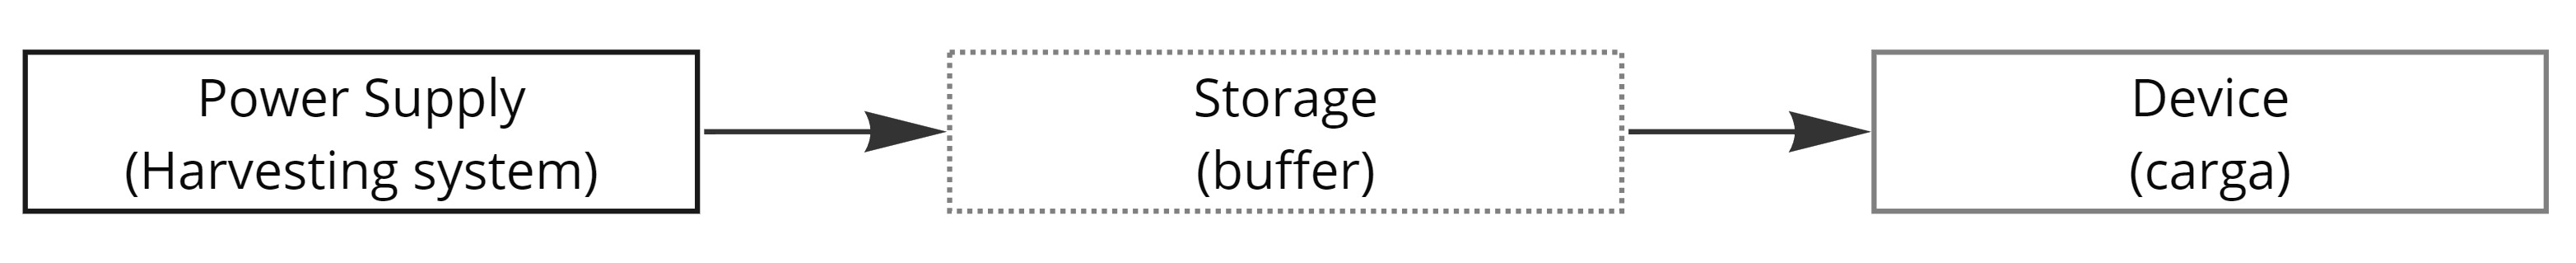
\includegraphics[width=0.7\linewidth]{Imagens/cap2/cap2harvest_store_use}	
	
	Fonte: adaptado de \cite{sudevalayam_energy_2011} 
\end{figure}

A visão do cenário acima proporciona ao node a capacidade de manter seus níveis de operação, abstraindo em algum nível as variações de energia coletada. Pois seja $P_{s}(t)$ a entrada energética em dado momento e  $P_{c}(t)$ a energia consumida nos ciclos de carga, é possível encontrar a dinâmica apresentada na Figura \ref{fig:cap2energyneutraloperation}, em momento de abundancia energética o node pode armazenar a energia que supera a quantidade necessária para sua operação em decorrência de que em momentos de escassez, possa fazer uso dessa energia suplementando sua necessidade. 


Operações neutro-energéticas carregam dois princípios que são apresentados no trabalho seminal de \cite{kansal_power_2007}: Manter-se operacional mesmo em cenários onde a quantidade de energia coletada fosse durante muito tempo, inferior ao necessário e como garantir que, encontrado em um ambiente de coleta seja possível obter performance esperada tolerando variações da energia coletada. 

\begin{figure}[H]
	\centering
	\caption{Dinâmicas de operação com coleta de energia} \label{fig:dinamicas}
	\begin{subfigure}{0.49\textwidth}
		\caption{Operação com buffer intermediário.}
		\label{fig:cap2energyneutraloperation}
		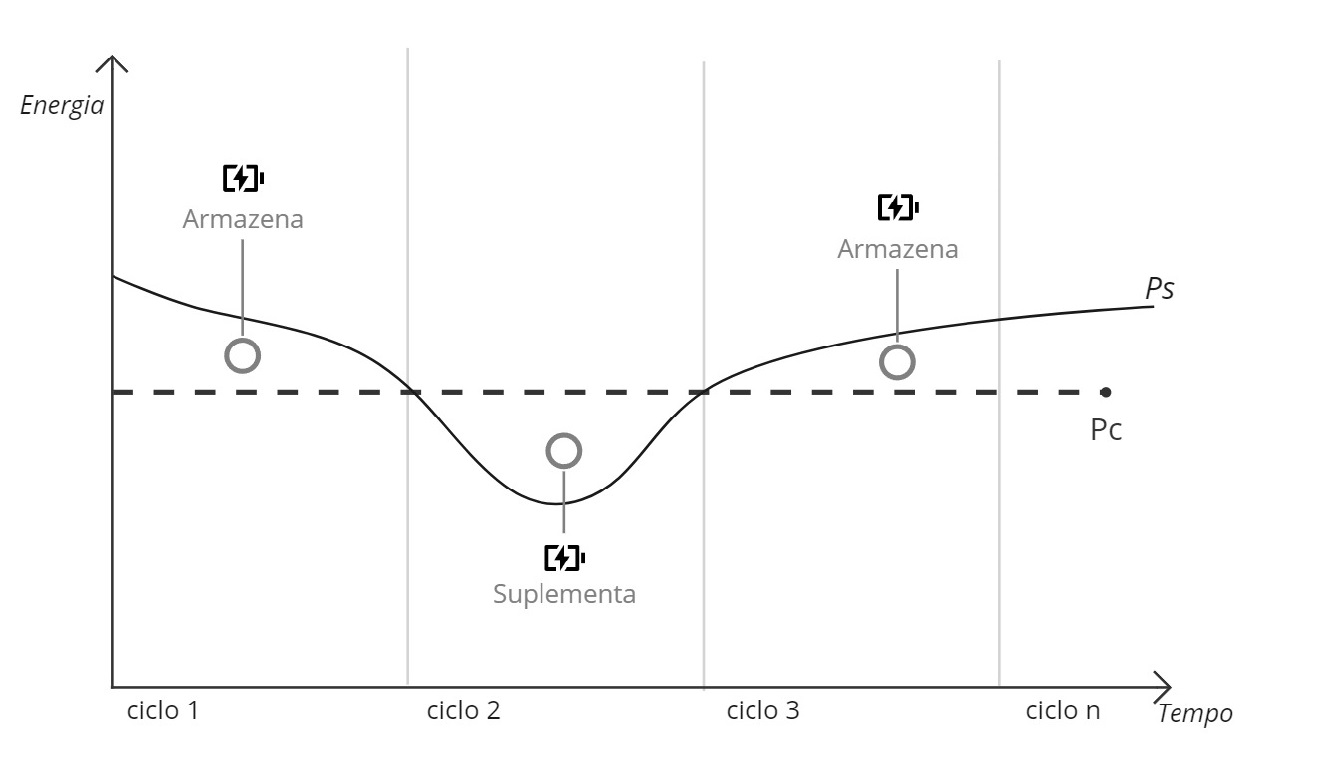
\includegraphics[width=\linewidth]{Imagens/cap2/cap2energyneutraloperation.jpg}	
	\end{subfigure}%
	\hspace*{\fill}  
	\begin{subfigure}{0.49\textwidth}
		\caption{Operação Power-Neutral.}
		\label{fig:cap2powerneutraloperation}
		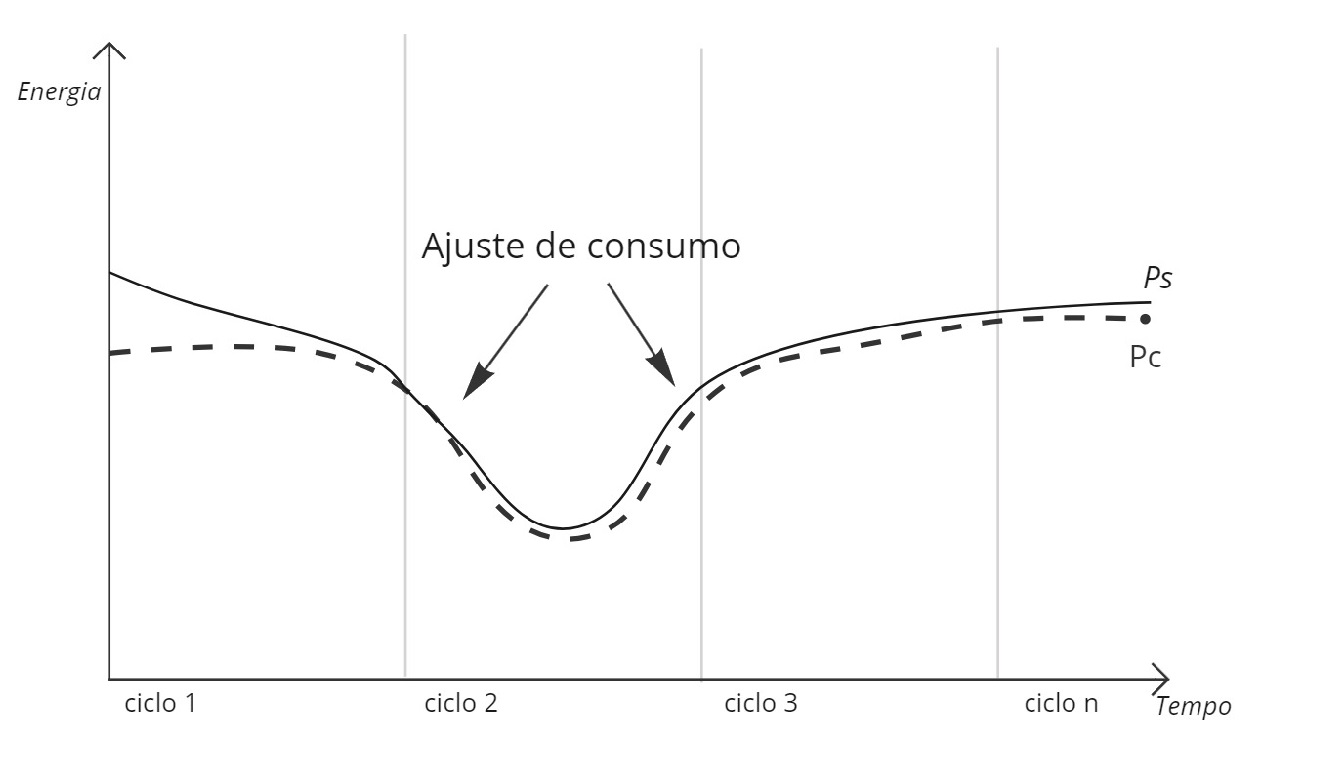
\includegraphics[width=\linewidth]{Imagens/cap2/cap2powerneutraloperation.jpg}
	\end{subfigure}%
	\hspace*{\fill}   
	
	Fonte: elaborado pelo autor.
\end{figure}

Sendo assim, uma operação neutro-energética implica em manter sua a performance durante os ciclos de trabalho garantindo que o node não sofra por esgotamento energético. Busca-se perpetuar sua operação mediante uso da reserva energética ou adaptação motivada a expectativa de recurso futuro \cite{sudevalayam_energy_2011}. Desta forma, o dispositivo favorecido pode prolongar sua operação mesmo em decorrência da indisponibilidade ou insuficiência de fonte energética.

É importante destacar que este modo de operação serviu como base para diversos avanços em computação dirigida a energia sobretudo em redes constituídas tipicamente com sensores embarcados, autônomos e distribuídos espacialmente, \acf{WSN}. Além disso, os conceitos de operação-neutra e a teoria de coleta energética foram fundamentais para o que posteriormente foi detalhado em referencia ao seminal \cite{merrett_energy-driven_2017}, introdutório ao modelo \acf{PNO}.



\subsection{Operação Power-Neutral}
A capacidade de um dispositivo em coletar energia do meio introduz inúmeros desafios principalmente enquanto ao movimento de coleta-transforma-usa e também quanto a previsibilidade de oferta. A abordagem ilustrada na Figura \ref{fig:cap2harveststoreuse} é tipica de um sistema que faz uso de um \textit{buffer} intermediário com o fundamento de que caso corretamente projetado, o subsistema aparentemente operara semelhante a um sistema alimentado por baterias. Todavia, em muitos casos, todo aparato embarcado ao dispositivo para garantir essas características incrementam custo, volume e complexidade, além disso, se mal projetado poderá dispor-se de comportamento não confiável.

Segundo \cite{merrett_energy-driven_2017}, os esforços para projetar um sistema com capacidade de coleta energética devem agora considerar os casos onde há impossibilidade de embarcar um componente de armazenamento energético intermediário. Portanto, sistemas com essa indisponibilidade deverão buscar um modo de operação \textit{Power-Neutral} conforme Figura \ref{fig:cap2powerneutraloperation}.

Operação \textit{Power-Neutral} descreve as ações em busca de cooperação com as dinâmicas de coleta energética através da adaptação seu consumo energético para manter-se operacional em acordo com recurso disponível \cite{sliper_energy-driven_2020}, minimizando ou até mesmo dispensando a necessidade de armazenamento intermediário. De toda maneira, é preciso considerar que caso a energia coletada seja inferior ao minimo necessário, cenário de esgotamento, conduzirá o dispositivo ao sumário desligamento.


\section{Redes IoT}
\label{cap2:iot}
\begin{itemize}
	\item Revisão da literatura sobre os diferentes componentes de consumo de energia em dispositivos IoT, incluindo processadores, transmissores de rádio, sensores e circuitos de controle de energia.
	\item Abordagens e modelos para estimar e prever o consumo de energia em dispositivos IoT.
	\item Leitura Pertinente: referencia de estudos sobre técnicas e estratégias para otimizar o consumo de energia em dispositivos IoT, assim como esquemas de gerenciamento de energia em redes IoT.
\end{itemize}

\section{Throttling: Padrão de Controle de Comportamento em Ambientes Distribuídos}
\label{cap2:throttling}

Como ponto de partida, é preciso destacar a importância da adoção de padrões \textit{patterns}, em especial em sistemas distribuídos. Tais padrões carregam aspectos intrínsecos a experiencia adquirida mediante a recorrência de uma dada solução à heterogeneidade de problemas apresentados, fomando o conjunto de situações onde dado padrão surge como possibilidade de resposta aos desafios encontrados. Em \cite{burns_designing_nodate}, particularmente no cenário de computação distribuído é evidenciado que apesar da diversidade de possibilidades para um dito negócio, o modo como é concebido, construído, desenvolvido e os problemas encontrados sobretudo os  aspectos não funcionais como escalabilidade, confiabilidade ou disponibilidade são notavelmente recorrentes e semelhantes. 

Problemas são semelhantes


\begin{itemize}
	\item Conceituação de throttling e sua aplicação em sistemas computacionais distribuídos.
	\item Exploração de diferentes técnicas de throttling e seus efeitos sobre o consumo de energia e desempenho do sistema em cenários como redes IoT.
	\item Leitura Pertinente: referencias de estudos que aborda o uso de throttling em ambientes distribuídos e sua influência na eficiência energética.
\end{itemize}

\section{Taxonomia}
\label{cap2:taxonomia}

Taxonomia refere-se ao sistema de classificação e organização de coisas. Seu modelo consiste em sistematicamente apresentar os elementos de um campo de estudo, categorizados e por conseguinte classificados de modo a apresentar os elementos dispostos em estrutura adequada.

O mapeamento sistemático apresentado em \cite{usman_taxonomies_2017}, trata dos métodos e da aplicação de taxonomias em campos da engenharia de software. O procedimento classificação, definem como as instancias de um tema podem ser atribuídos a classes ou categorias. Para uma taxonomia, tais elementos podem estar relacionados e dependentes entre si. Por sua vez, é possível classificar de duas maneiras: Quantitativamente, onde os procedimentos de classificação são baseados em escalas numéricas ou Qualitativa onde uma escala nominal que expresse a categoria será utilizada. Sua estrutura, segundo \cite{kwasnik_role_nodate} poderá ser definida em quatro visões de descobrimento do conhecimento.

\textbf{Hierárquico}, aqui a taxonomia é estruturada como uma única classe superior (superclasse) que abrange suas subclasses e sequencialmente as possíveis extensões destas, formando um encadeamento hierárquico entre os elementos desde o originário até os derradeiros derivados. Este modelo procura garantir a exclusão mutua entre os envolvidos além do aspecto de relacionamento hereditário, por isso não é recomendado em situações onde uma pesquisa precisa incluir múltiplos e diversos critérios de diferenciação. Por fim, o autor considera que para esta representação é mandatório bom conhecimento sobre o assunto a ser classificado., pois suas classes e critérios de separação precisam ser conhecidos desde o inicio.

\textbf{Árvore} similar ao modelo hierárquico, todavia em uma estrutura árvore não existe um relacionamento do tipo herança. Aqui, o tipo de classificação que busca-se é a relação causa-efeito, processo-produto ou parte-todo. Pode-se usar a estrutura arvore para mostrar a decomposição de um tema em seus aspectos. Por exemplo, a representação em árvore parte-todo do relacionamento entre um país, seus estados e por fim, municípios. Estruturas árvores e hierárquicas compartilham das mesmas limitações.

\textbf{Paradigma}, conduz a taxonomia para a capacidade de um relacionamento bi-direcional entre as classes estas, por sua vez, podem ser descritas pela combinação de dois atributos. Uma proposta de visualização para taxonomias desse tipo é a capacidade de expressar-se com matrizes bi-dimensionais cujo seus vértices apresentam os atributos de interesse.

\textbf{Facetada}, esta estrutura taxonômica permite observar os assuntos classificados sob múltiplas perspectivas (facetas). O indicador fundamental em utilizar uma análise facetada é a necessidade de visualizar mais de uma perspectiva de uma entidade complexa. Cada faceta é independente e pode ter suas próprias classes, permitindo a evolução de cada uma dentro da sua perspectiva. Análise facetada é adequada para campos de conhecimento relativamente novos em constante evolução, dado que não é necessário ter o completo conhecimento do objeto de estudo. Em todo caso, pode ser desafiador encontrar o conjunto inicial de facetas para a taxonomia de modo que sejam independentes e sem aparente relacionamento significativo entre as facetas.

No trabalho \cite{smite_empirically_2014}, são indicados três mecanismos como validadores de uma taxonomia: a demonstração ortogonal de perpendicularidade e dimensões das classes é demonstrada; análise de desempenho (\textit{Benchmarking}), onde a taxonomia pode ser comparada com outros esquemas de classificação similares; e, por fim, a demonstração de utilidade, validada por estudo de caso ou experimentação.

O debate sobre qual visão escolher é crucial, pois interfere imediatamente sobre a maneira como representar classes e interações. Quanto à aplicação prática para Engenharia de Software, ao adotar o uso de uma taxonomia, temos os agentes facilitadores para atividades de classificar e organizar o conhecimento de uma área \cite{usman_taxonomies_2017}, auxiliando no desdobramento e acomodação do objeto de estudo, elucidação e identificação de oportunidades e trabalhos futuros.






\section{Considerações Finais}
 \label{cap2:consideracoesFinais}
\begin{itemize}
	\item Síntese dos principais pontos discutidos no referencial teórico.
	\item Apontamento para a relevância desses conceitos na elaboração e implementação do projeto proposto.
\end{itemize}
	

\blindtext[2]
